\documentclass[envcountsame,envcountchap]{svmono}
% Import fontspec package for font management
\usepackage{fontspec}

% Set main font (example using "Times New Roman")
%\setmainfont{Baskerville}

\usepackage{parskip}
\usepackage{makeidx}    % allows index generation
\usepackage{graphicx}   % standard LaTeX graphics tool when including figure files
\usepackage{subcaption} % per più figure sulla stessa riga
\usepackage{wrapfig}
\usepackage{multicol}
\usepackage{booktabs}
\usepackage{latexsym}
\usepackage[italian]{babel}
\usepackage{blindtext}
\usepackage{xcolor}
\usepackage{multirow}
\usepackage{multicol}
\usepackage{float}
\usepackage{minted}
\usepackage[hyphens]{url}
\usepackage{acronym}
\usepackage{natbib}
\usepackage{array}
\usepackage{lscape}
\usepackage{hyperref} % serve per inserire link nel testo, 
% utile solo per documenti non destinati alla stampa


\setlength{\textwidth}{12.7cm}
\setlength{\textheight}{20.0cm}
\setlength{\oddsidemargin}{3.50cm}
\setlength {\evensidemargin}{-0.3cm}  %foglio a destra 0.06
\setlength {\topmargin}{-1cm}

\renewcommand\definitionname{Definizione}
\renewcommand\theoremname{Teorema}
\renewcommand\propositionname{Proposizione}
\renewcommand\corollaryname{Corollario}
\renewcommand\examplename{Esempio}




\def\punto{\hspace*{\fill}\Box}


\makeindex             % used for the subject index
                       % please use the style svind.ist with
                       % your makeindex program

%%%%%%%%%%%%%%%%%%%%%%%%%%%%%%%%%%%%%%%%%%%%%%%%%%%%%%%%%%%%%%%%%%%%%
\date{}
\begin{document}

%\maketitle


\pagenumbering{Roman}
%\setcounter{page}{5}

\frontmatter

\begin{titlepage}

    \begin{center}

    \large{\bf Università degli Studi Mediterranea di Reggio Calabria}

    \vspace*{1mm}

    \large{Dipartimento di Ingegneria Civile, Energia, Ambiente e Materiali}

    \vspace*{1mm}

    \normalsize{Corso di Laurea in Ingegneria Industriale}

    \vspace*{1mm}

    \hspace*{-0mm}

    \rule{125mm}{.2mm}  %{lunghezza}{spessore}


    \vspace{18mm}

    \begin{figure}[h!]
        \centerline{
\includegraphics[width=3cm]{logounirc.png}}
    \end{figure}

    \vspace{5mm}

    \textbf{Tesi di Laurea}

    \vspace{5mm}

    %% TITOLO DELLA TESI
    \large{\bf Creazione di un modello \LaTeX\ aggiornato e semplificato per tesi di laurea.}

    \vspace{22mm}

    \begin{tabular}{lcl}
        {\large Relatore} & \ \hskip 2.2cm \ & {\large Candidato} \\
        \ & \ & \ \\
        {Alessandro Campolo} &                  & {Alessandro Campolo}\\
        \ & \ & \ \\
        {\large Correlatore} &               & \\ %commentare se assente
        \ & \ & \ \\
        {Alessandro Campolo} &               & \\ %commentare se assente
        \\
    \end{tabular}

    \rule{125mm}{.2mm}

    \textbf{Anno Accademico 2023-2024}
    \end{center}

\end{titlepage}

\newpage
\newpage
\cleardoublepage
\thispagestyle{empty}
\vspace*{\stretch{1}}
\begin{flushright}
\itshape
<DEDICA>
\end{flushright}
\vspace{\stretch{2}}
\cleardoublepage

\newpage

\thispagestyle{empty}

% questo aggiunge l'indice al documento
\tableofcontents

\listoffigures



\pagenumbering{arabic} \setcounter{page}{7}

\chapter*{Indice degli acronimi}
\markboth{Indice degli acronimi}{Indice degli acronimi}
\begin{acronym}[WYSIWYM]
    % gli acronimi devono essere ordinati manualmente
    \acro{DICEAM}{Dipartimento di Ingegneria Civile, dell'Energia, dell'Ambiente e dei Materiali}
    \acro{DIIES}{Dipartimento di Ingegneria dell'Informazione, delle Infrastrutture e dell'Energia Sostenibile}
    \acro{DiGiES}{Dipartimento di Giurisprudenza, Economia e Scienze Umane}
    \acro{dArTe}{Dipartimento di Architettura e Territorio}
    \acro{PAU}{Dipartimento di Patrimonio, Architettura e Urbanistica}
\end{acronym}



% il motivo dei seguenti tre comandi è di creare un nuovo capitolo regolare, ma senza numero
\chapter*{Introduzione} \label{introduzione}
% l'asterisco crea un capitolo non numerato, non presente nell'indice
% e senza titolo in intestazione e piè di pagina
\addcontentsline{toc}{chapter}{Introduzione}
% addcontentsline aggiunge una voce all'indice
\markboth{Introduzione}{Introduzione}
% markboth imposta intestazione e piè di pagina

\vspace{2cm}

\hfill \textit{Introduzione al documento}

\vspace{0.5cm}


Il presente lavoro intende essere un modello di tesi del Dipartimento DICEAM 
(per l'esempio è stato usato il corso di Ingegneria Industriale).

Nel corso della trattazione verranno illustrati:
\begin{itemize}
    \item Installazione e configurazione di:
        \begin{itemize}
            \item TeX Live
            \item Visual Studio Code
            \item Estensione Latex Workshop per Visual Studio Code
        \end{itemize}
    \item Introduzione ai sistemi di controllo versione:
        \begin{itemize}
            \item git
            \item GitHub
            \item Fork e modifica di una repository
        \end{itemize}
    \item Esempi di elementi di \LaTeX\ come:
        \begin{itemize}
            \item immagini
            \item elenchi
            \item bibliografia
            \item tabelle
            \item spazi, righe e pagine
        \end{itemize}
\end{itemize}
  



\mainmatter%%%%%%%%%%%%%%%%%%%%%%%%%%%%%%%%%%%%%%%%%%%%%%%%%%%%%%%


\chapter{Preparazione dell'ambiente} \label{Cap.1}

\vspace{2cm}

\begin{flushright}
\textit{Installazione e configurazione del compilatore\\ TeX Live e dell'editor Visual Studio Code}
\end{flushright}

\vspace{0.5cm}

L'installazione dei programmi verrà documentata per le tre principali piattaforme
\begin{itemize}
    \item Windows
    \item MacOS
    \item Linux e Unix-like
\end{itemize}

\section{TeX Live}
Essendo il processo più lungo, è consigliabile cominciare con l'installazione di TeX Live.

\subsection{Windows}
Per l'installazione su Windows scaricare l'installer da \url{https://mirror.ctan.org/systems/texlive/tlnet/install-tl-windows.exe}.

L'installer è firmato con una chiave non registrata in Windows, di conseguenza SmartScreen visualizzerà un avviso,
l'installer è completamente sicuro ed è possibile ignorare questo avviso.
\begin{figure}[H]
    \centering
    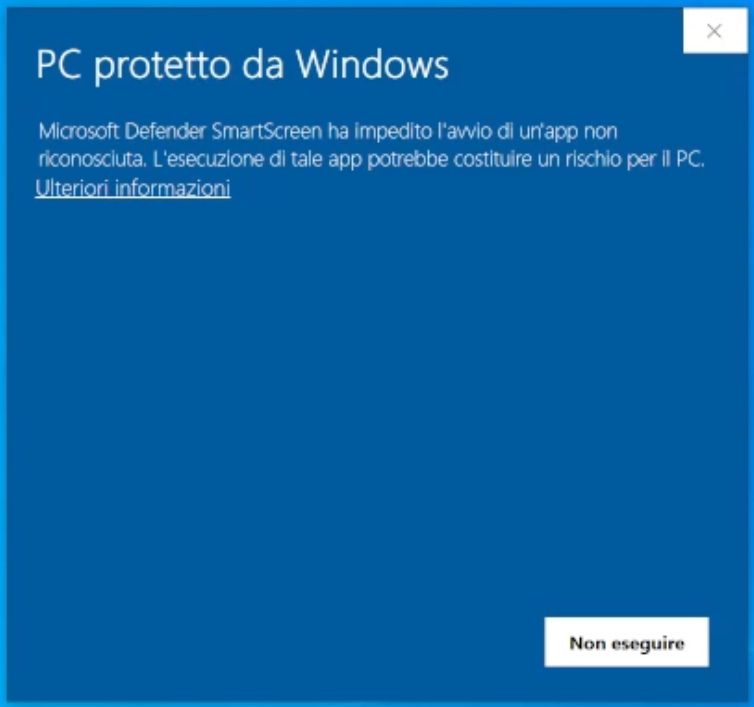
\includegraphics[width=0.5\linewidth]{images/texlive/win/1_smart_screen.png}
    \caption{Avviso di SmartScreen}
    \label{avviso_smart_screen}
\end{figure}
Cliccare "Ulteriori informazioni" per mostrare il pulsante "Esegui comunque" e cliccarlo.
\begin{figure}[H]
    \centering
    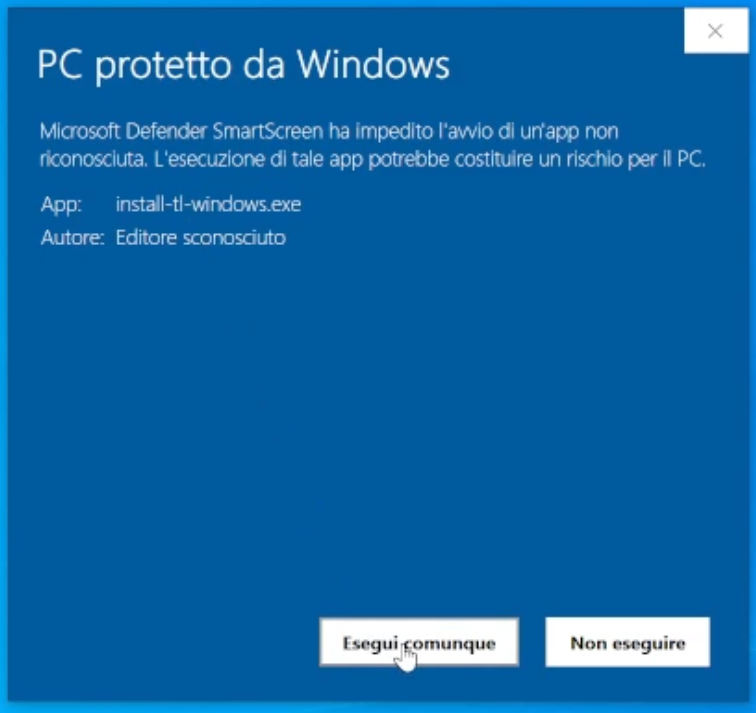
\includegraphics[width=0.5\linewidth]{images/texlive/win/2_smart_screen_2.png}
    \caption{Ulteriori informazioni di SmartScreen}
    \label{info_smart_screen}
\end{figure}
Nella prima schermata dell'installer scegliere "Install", poi premere "Next" e infine "Install".
\begin{figure}[H]
    \begin{subfigure}{0.49\textwidth}
        \centering
        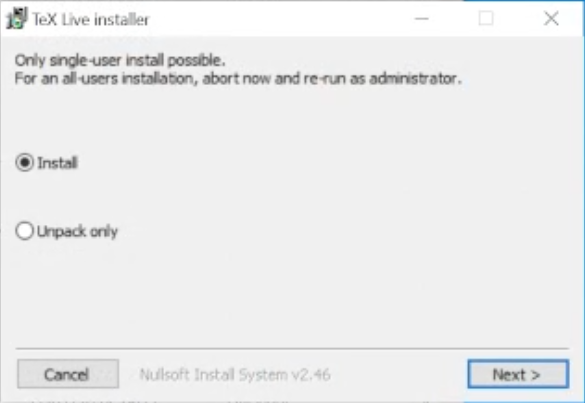
\includegraphics[width=\linewidth]{images/texlive/win/3_install_mode.png}
        \caption{Selezione modalità di installazione}
        \label{texlive_install_mode}
    \end{subfigure}
    \begin{subfigure}{0.49\textwidth}
        \centering
        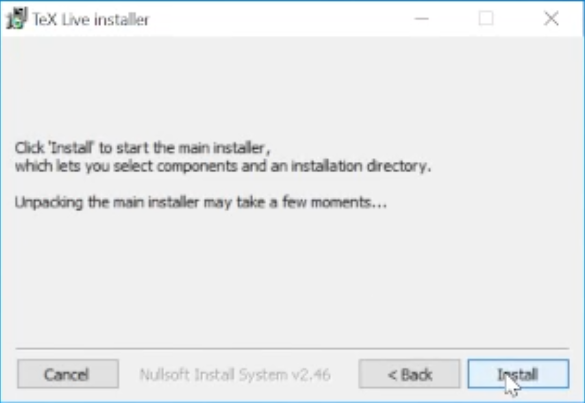
\includegraphics[width=\linewidth]{images/texlive/win/4_start_installer.png}
        \caption{Avvio del configuratore}
        \label{texlive_config}
    \end{subfigure}
\end{figure}
Nella schermata che si apre scegliere il mirror italiano dal menu a tendina.
\begin{figure}[H]
    \centering
    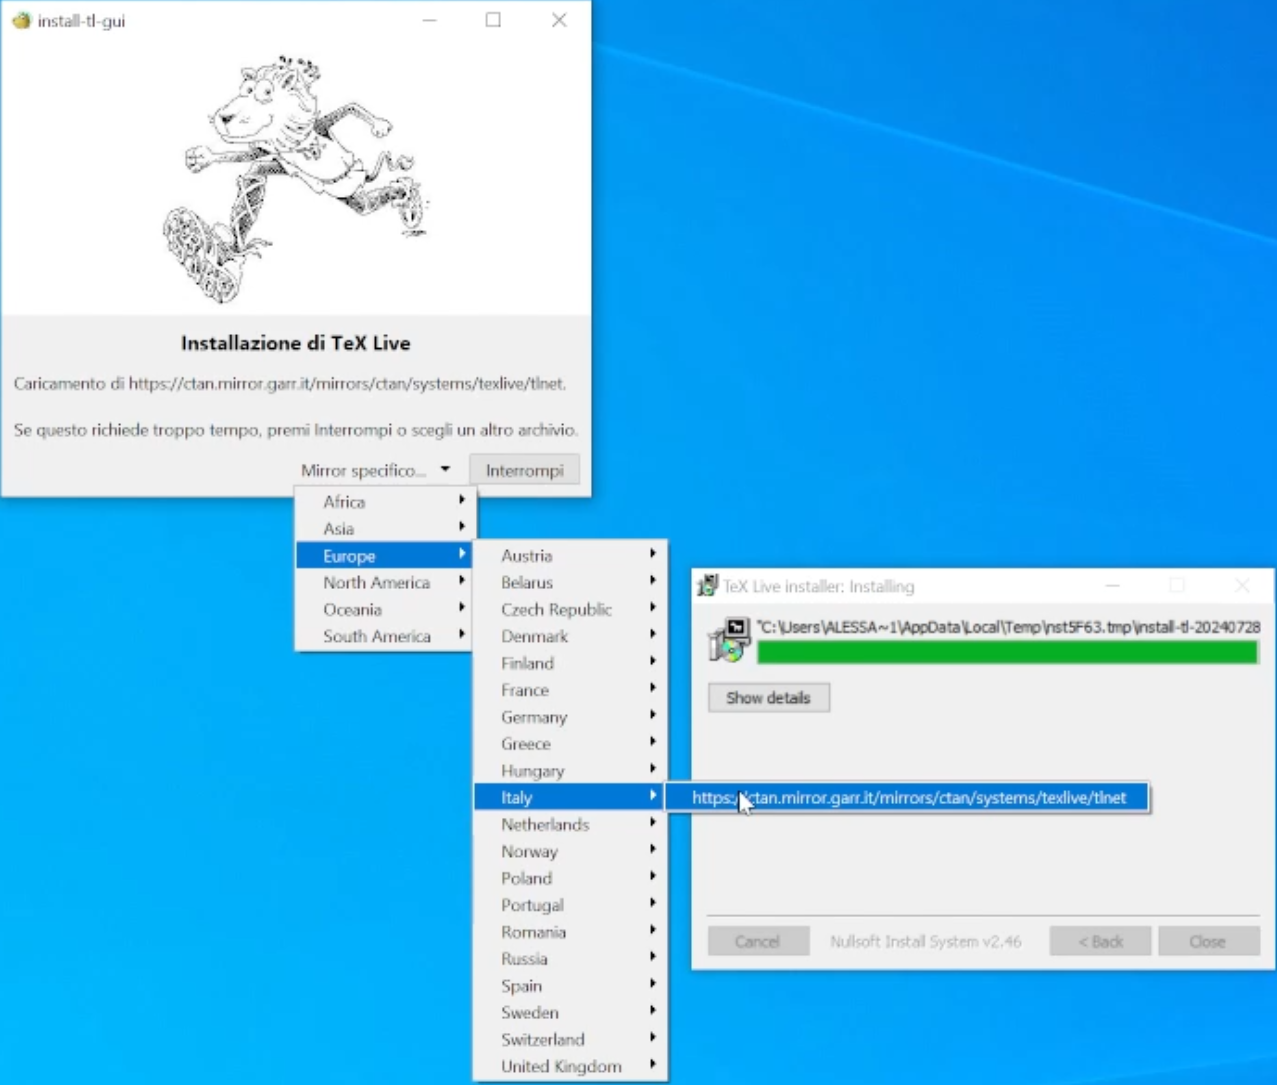
\includegraphics[width=0.95\linewidth]{images/texlive/win/6_mirror_select.png}
    \caption{Selezione del mirror}
    \label{texlive_mirror}
\end{figure}
Dal momento che si userà solo Visual Studio Code per la scrittura, è possibile escludere TeXworks dall'installazione.
Utenti più esperti possono usare le opzioni avanzate per selezionare manualmente i pacchetti da installare
e velocizzare l'installazione. Questa parte non è attualmente oggetto della documentazione e viene lasciata
come triviale esercizio per il lettore.
\begin{figure}[H]
    \centering
    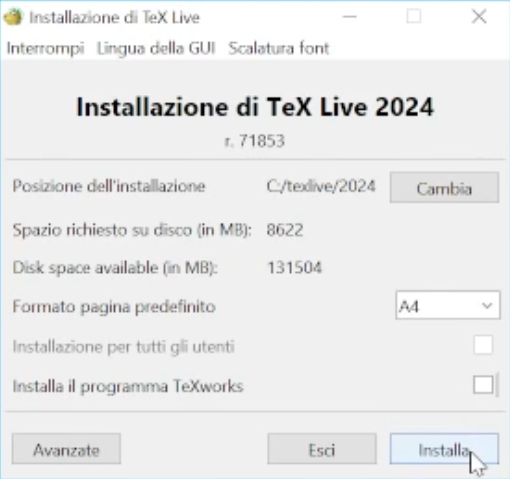
\includegraphics[width=0.8\linewidth]{images/texlive/win/7_configurator.png}
    \caption{Ulteriori configurazioni}
    \label{texlive_config_2}
\end{figure}
L'installazione di tutti i pacchetti può richiedere anche due ore, è possibile continuare a seguire i passaggi successivi di questa guida.
\begin{figure}[H]
    \begin{subfigure}{0.49\textwidth}
        \centering
        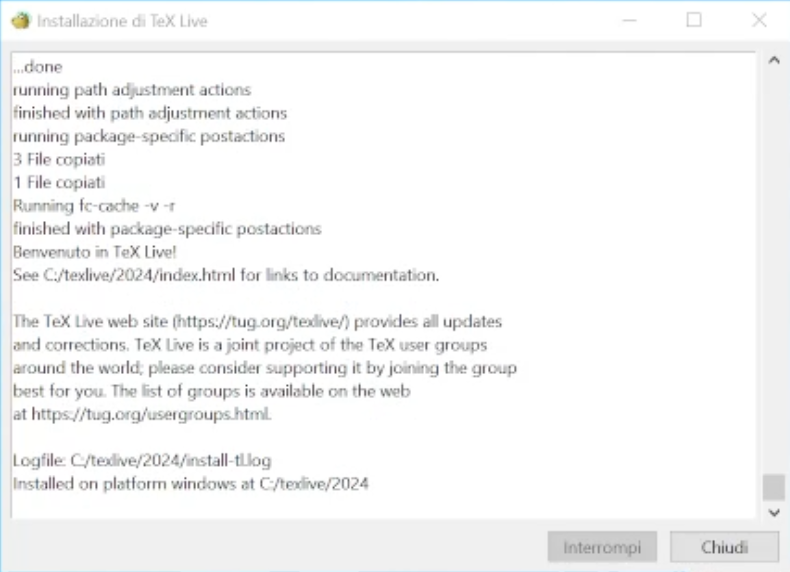
\includegraphics[width=\linewidth]{images/texlive/win/8_download_packages.png}
        \caption{Log di installazione}
        \label{texlive_install_log}
    \end{subfigure}
    \begin{subfigure}{0.49\textwidth}
        \centering
        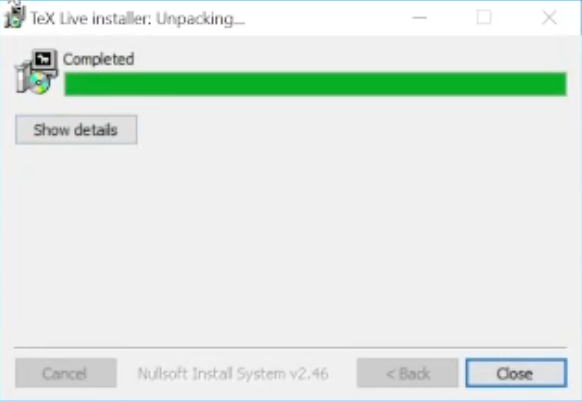
\includegraphics[width=\linewidth]{images/texlive/win/9_end_screen.png}
        \caption{Fine dell'installazione}
        \label{texlive_installato}
    \end{subfigure}
\end{figure}


\subsection{MacOS \citep{installMacTeX}}
Dopo il download di \url{https://mirror.ctan.org/systems/mac/mactex/MacTeX.pkg}, fare doppio clic per installarlo. Seguite le semplici istruzioni. L'installazione su un Macintosh recente richiede circa dieci minuti.

Il programma di installazione presenta:
\begin{itemize}
    \item una pagina di benvenuto
        \begin{figure}[H]
            \centering
            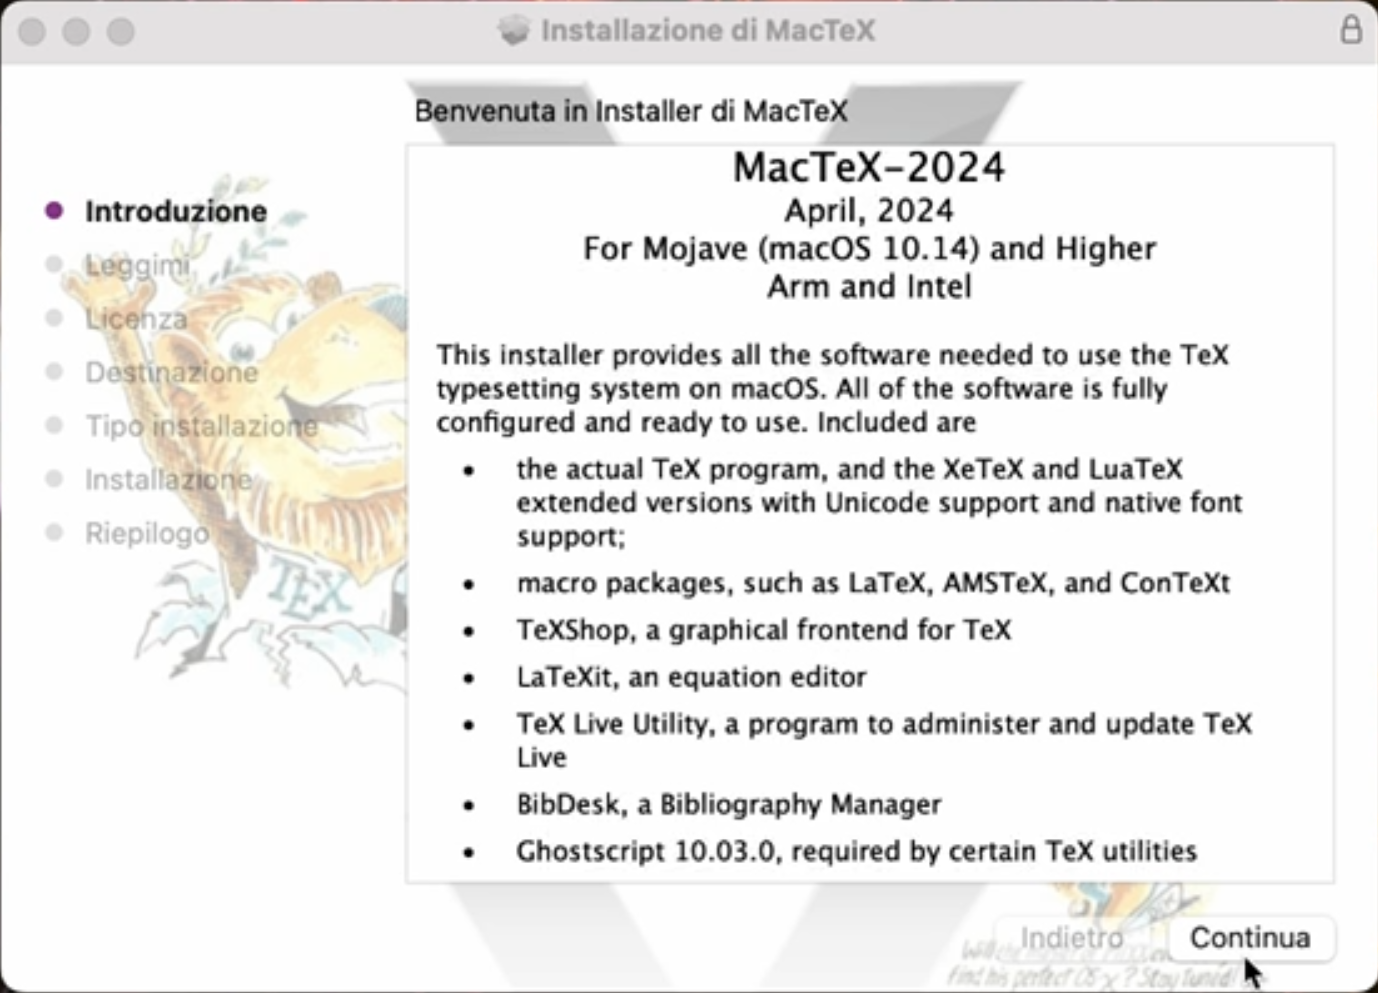
\includegraphics[width=0.5\linewidth]{images/texlive/mac/1_introduzione.png}
            \caption{MacTeX: Introduzione}
            \label{mactex_introduzione}
        \end{figure}
    \item una pagina ReadMe con ulteriori informazioni
        \begin{figure}[H]
            \centering
            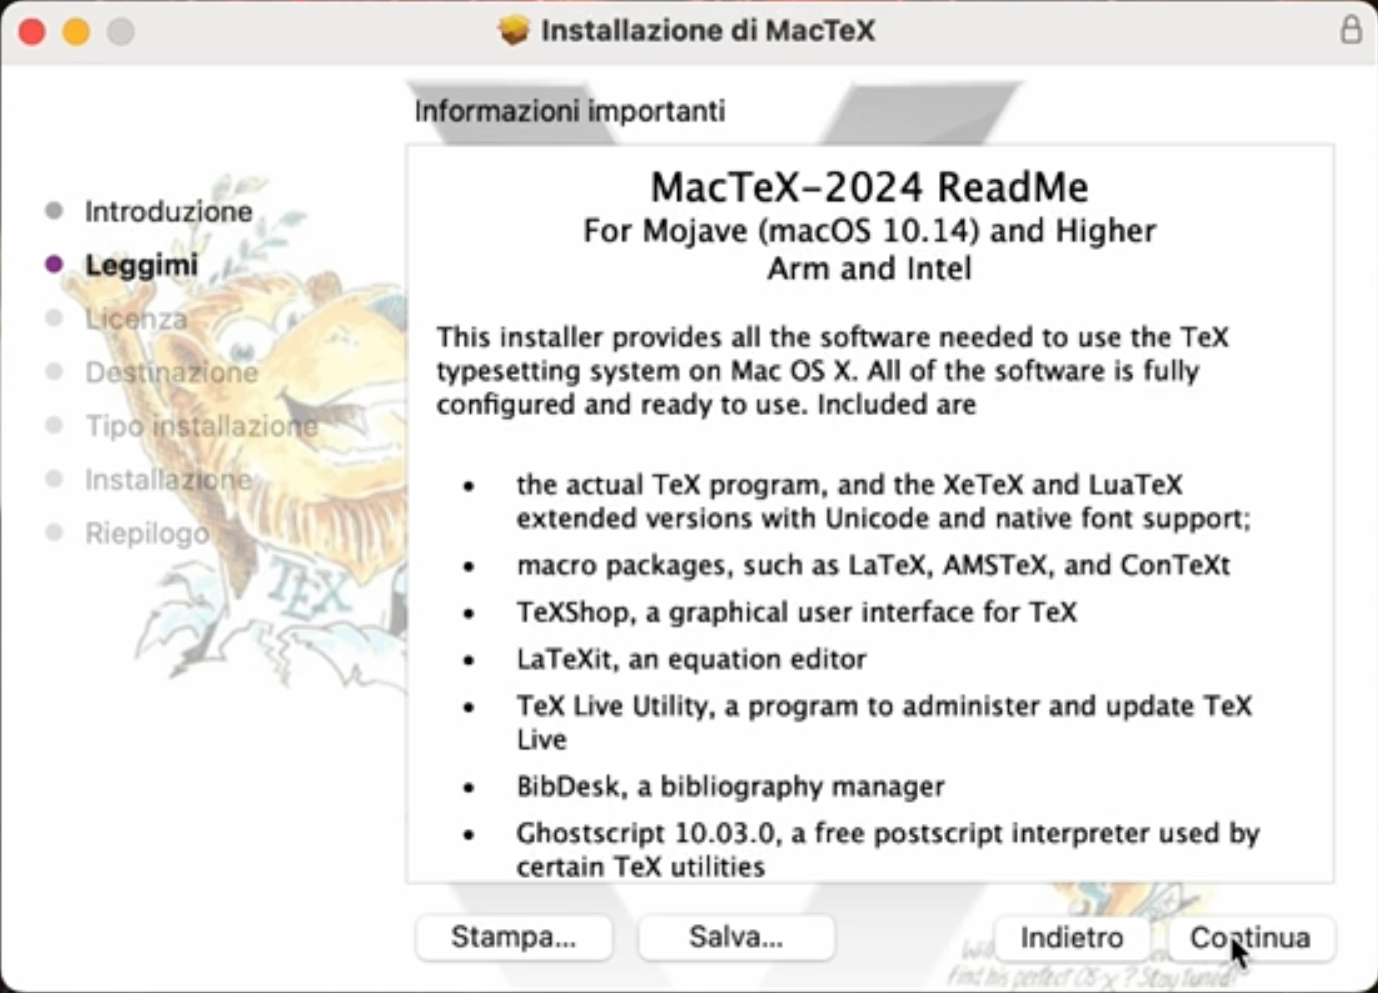
\includegraphics[width=0.5\linewidth]{images/texlive/mac/2_leggimi.png}
            \caption{MacTeX: Leggimi}
            \label{mactex_readme}
        \end{figure}
    \item una pagina di licenza software
        \begin{figure}[H]
            \centering
            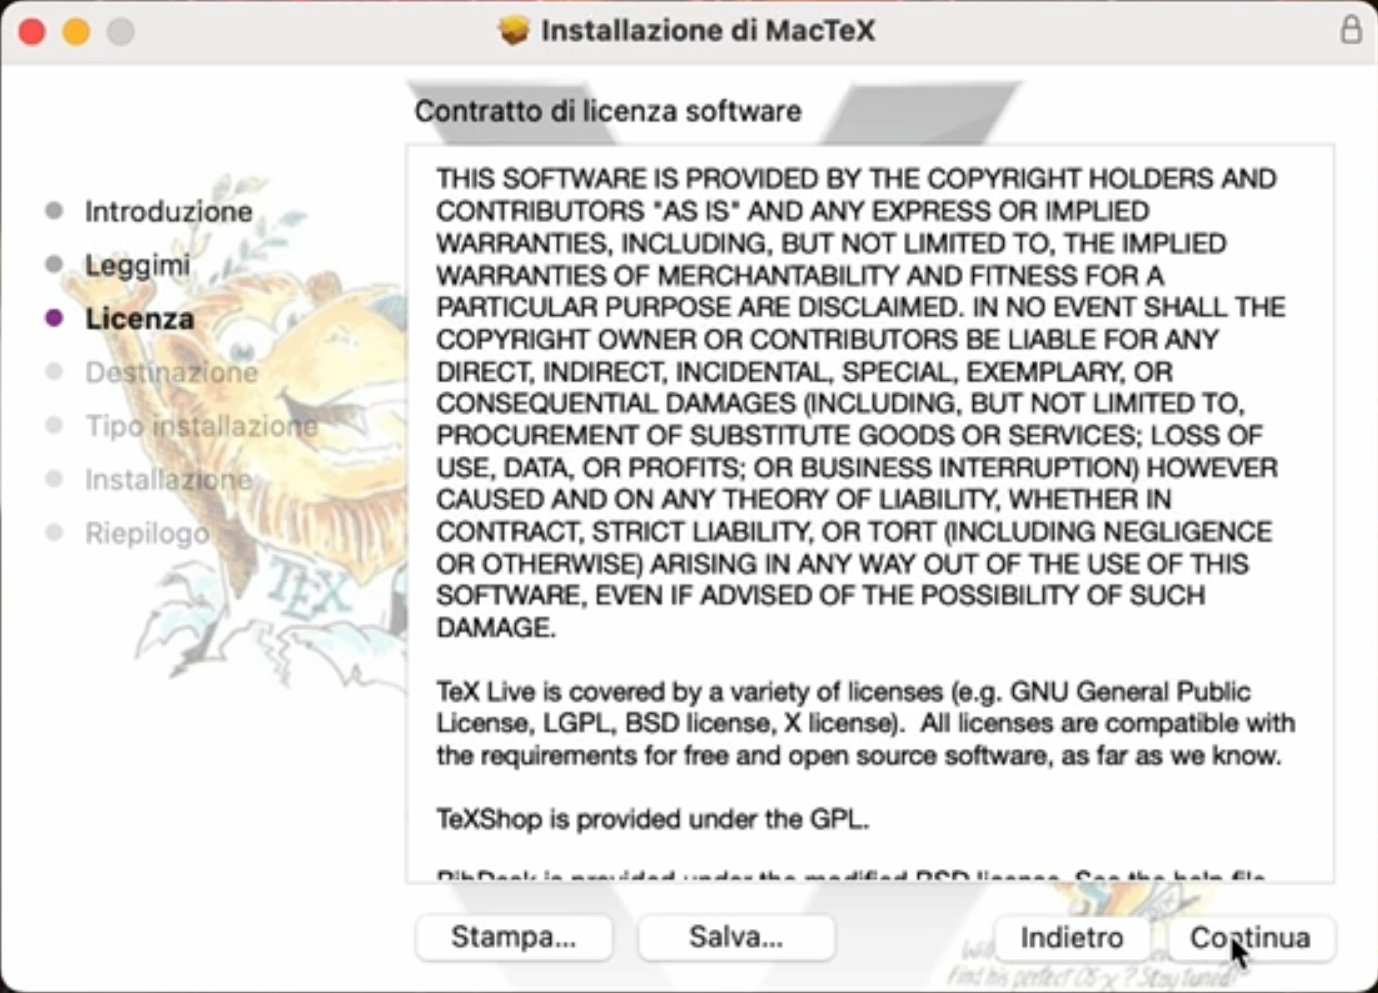
\includegraphics[width=0.5\linewidth]{images/texlive/mac/3_licenza.png}
            \caption{MacTeX: Licenza}
            \label{mactex_licenza}
        \end{figure}
    \item una finestra di dialogo per accettare la licenza
        \begin{figure}[H]
            \centering
            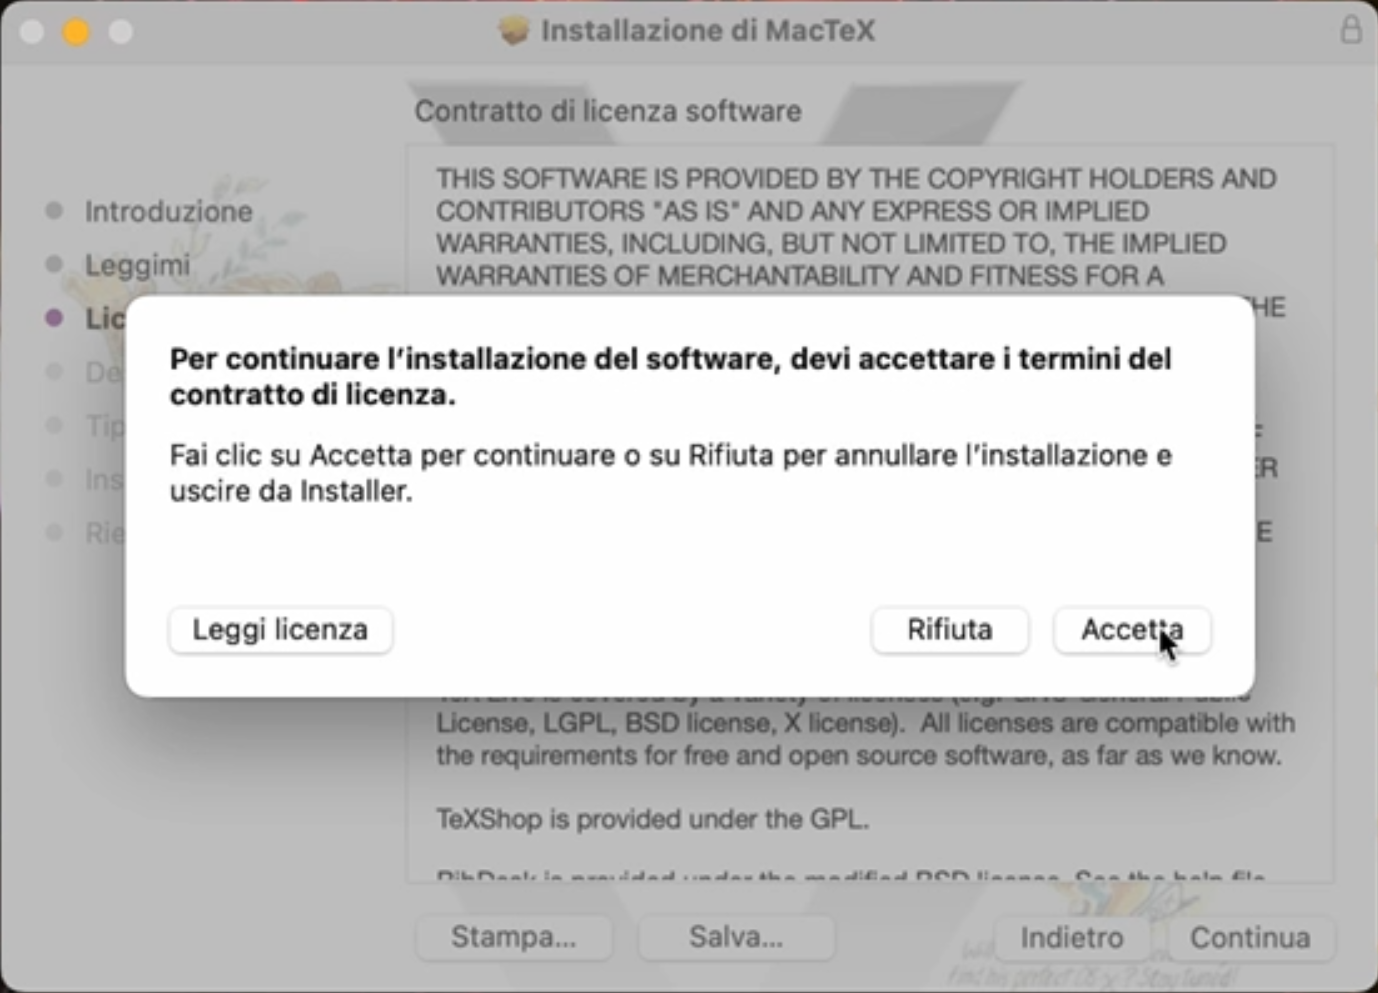
\includegraphics[width=0.5\linewidth]{images/texlive/mac/4_accettazione_licenza.png}
            \caption{MacTeX: Accettazione Licenza}
            \label{mactex_acc_licenza}
        \end{figure}
    \item una pagina di conferma della posizione di installazione
        \begin{figure}[H]
            \centering
            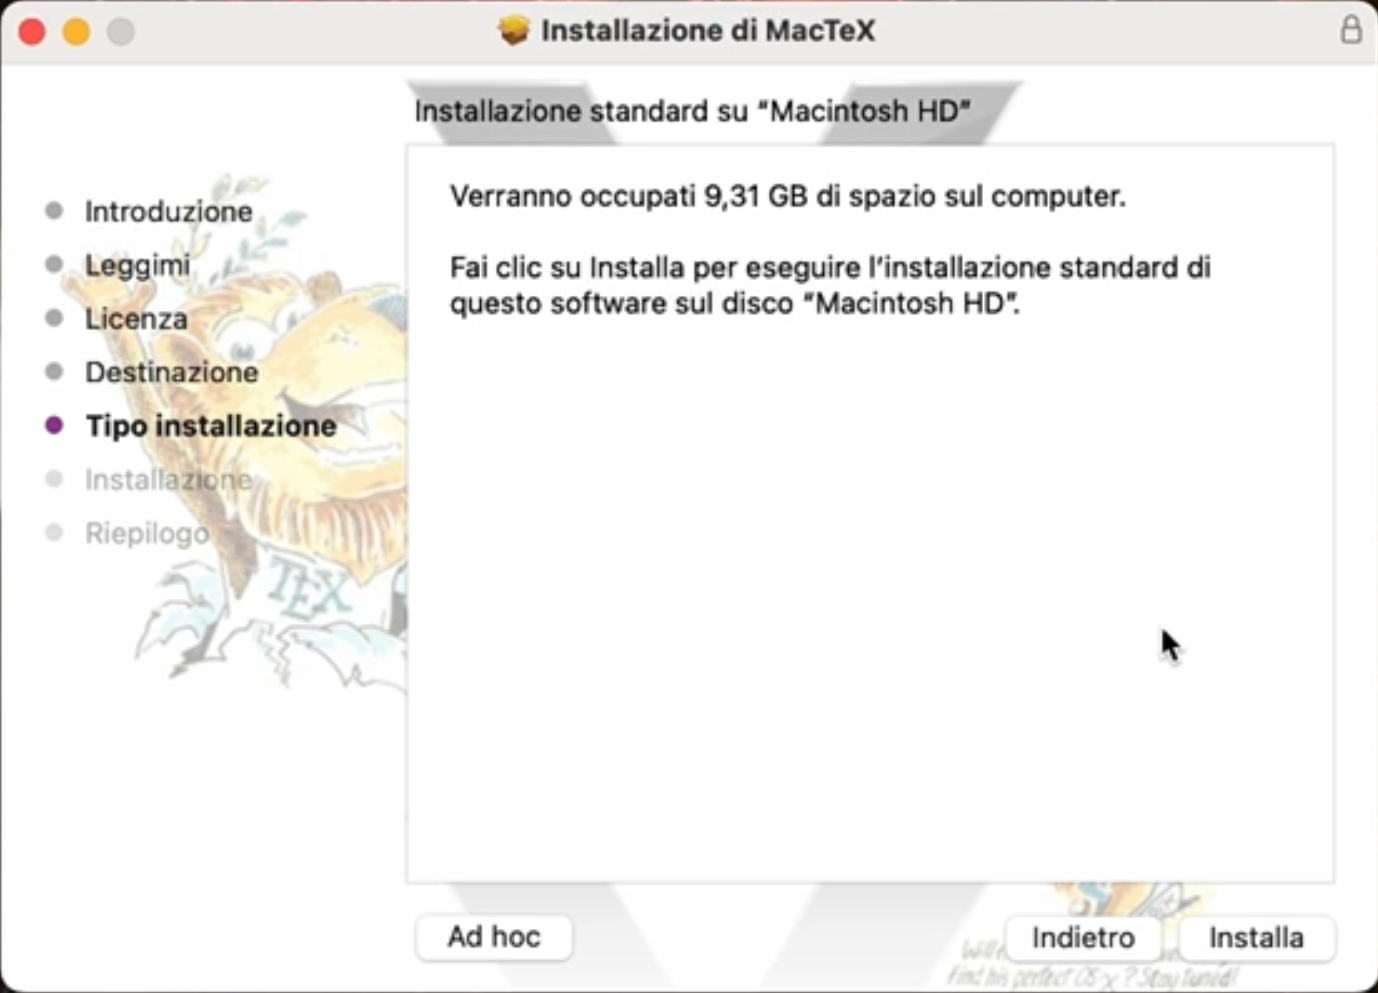
\includegraphics[width=0.5\linewidth]{images/texlive/mac/5_destinazione.png}
            \caption{MacTeX: Destinazione di installazione}
            \label{mactex_dest_installazione}
        \end{figure}
    \item una pagina con il progresso dell'installazione (confermare autenticandosi)
        \begin{figure}[H]
            \centering
            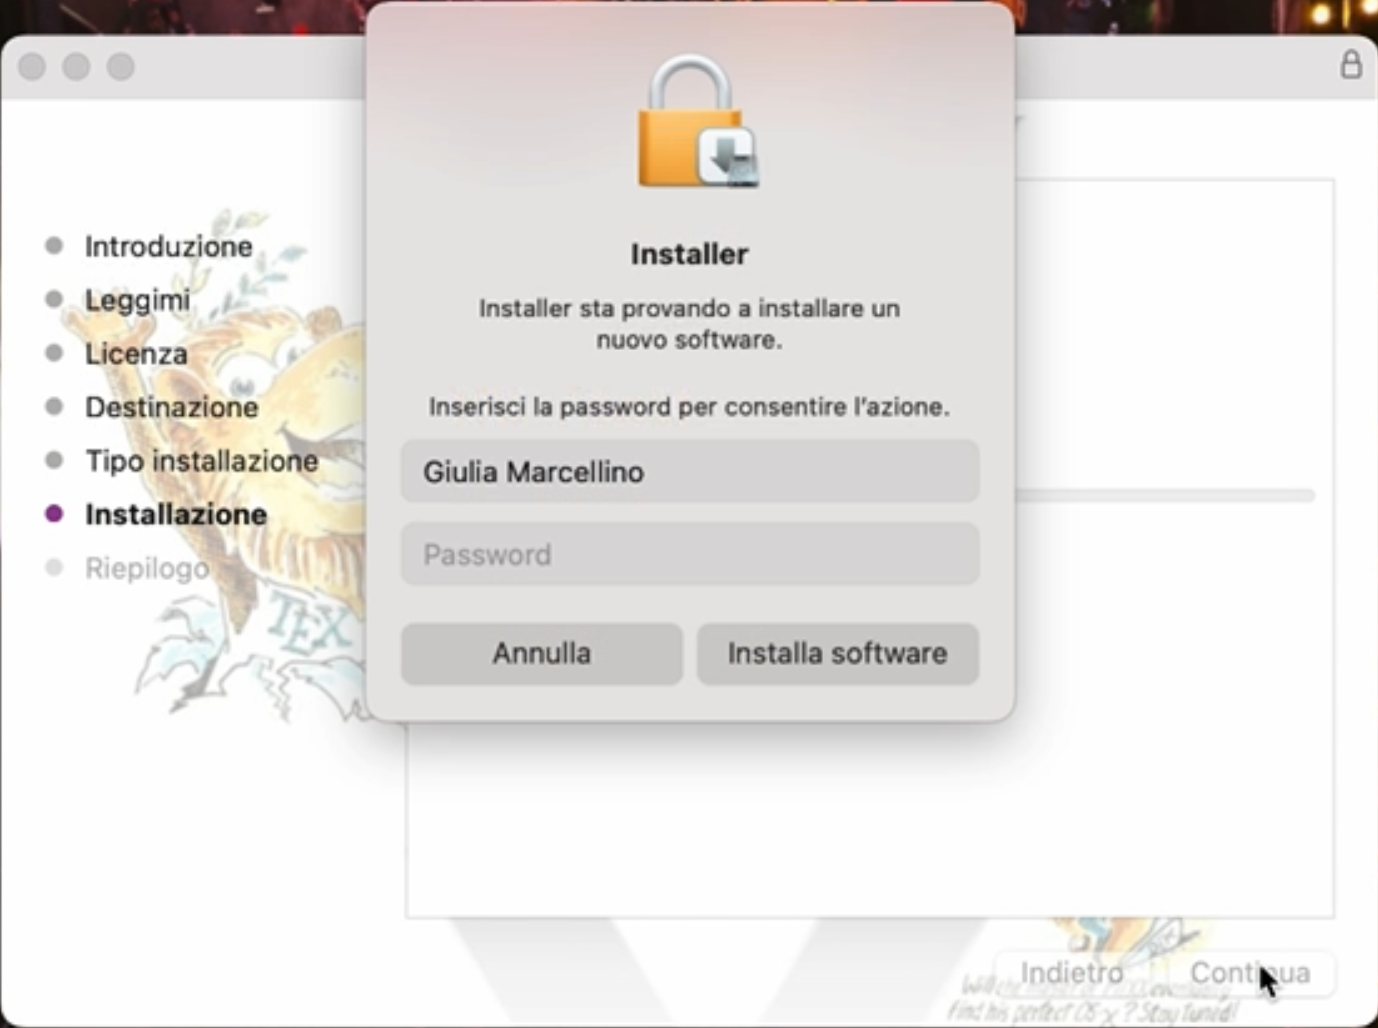
\includegraphics[width=0.5\linewidth]{images/texlive/mac/6_installazione.png}
            \caption{MacTeX: Autenticazione per l'installazione}
            \label{mactex_install_auth}
        \end{figure}
    \item una pagina finale
        \begin{figure}[H]
            \centering
            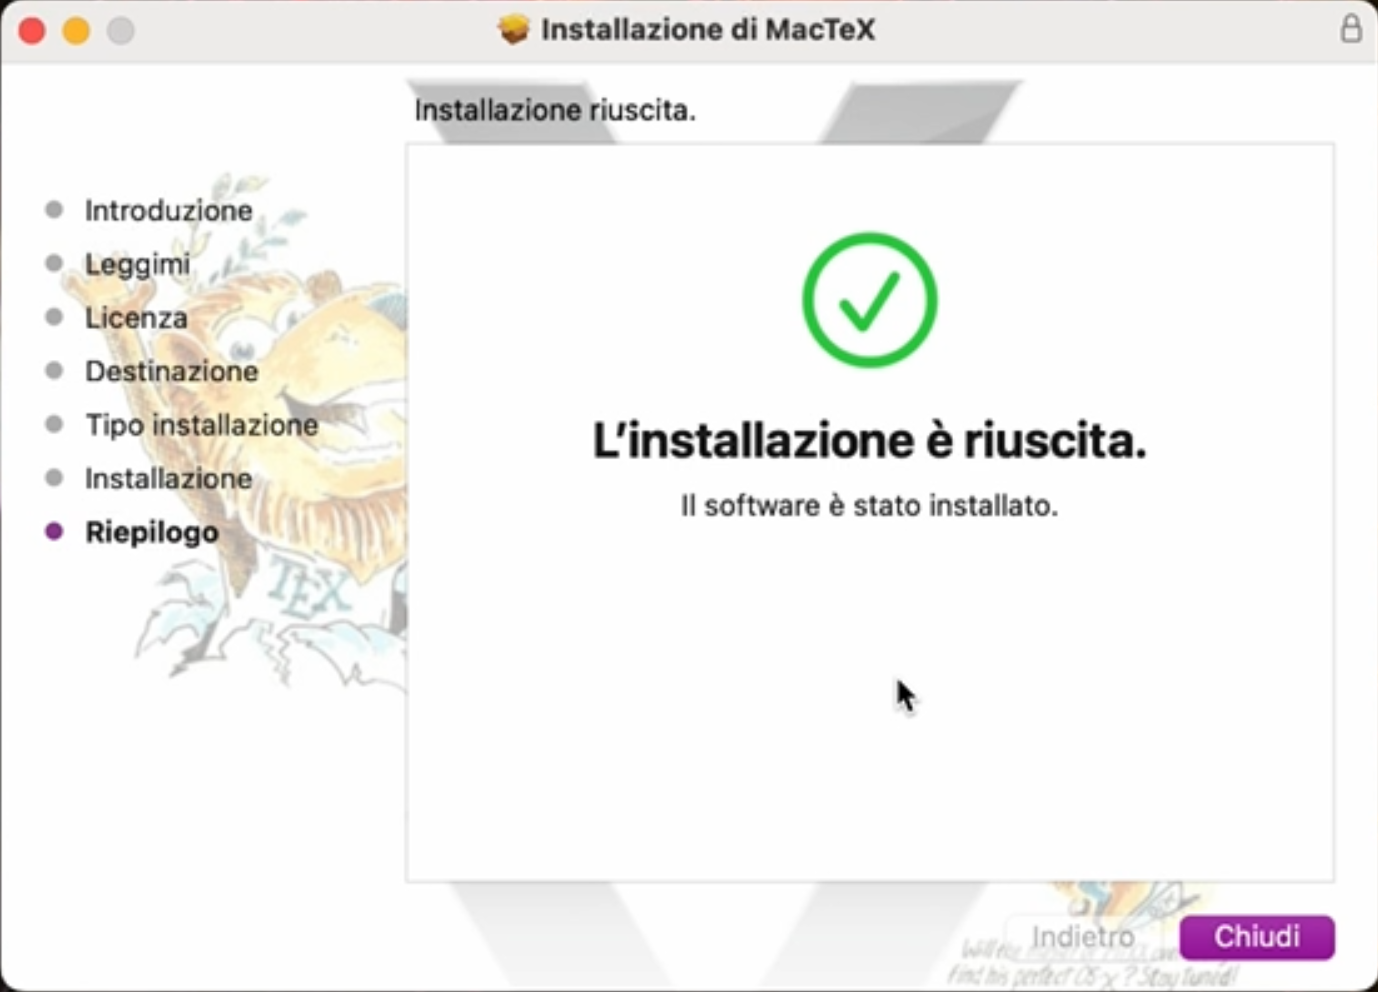
\includegraphics[width=0.5\linewidth]{images/texlive/mac/7_fine_installazione.png}
            \caption{MacTeX: Fine installazione}
            \label{mactex_fine_inst}
        \end{figure}
\end{itemize}

Al termine dell'installazione una finestra di dialogo chiede se si vuole eliminare l'installer,
spostarlo nel cestino per risparmiare spazio su disco.

\begin{figure}[H]
    \centering
    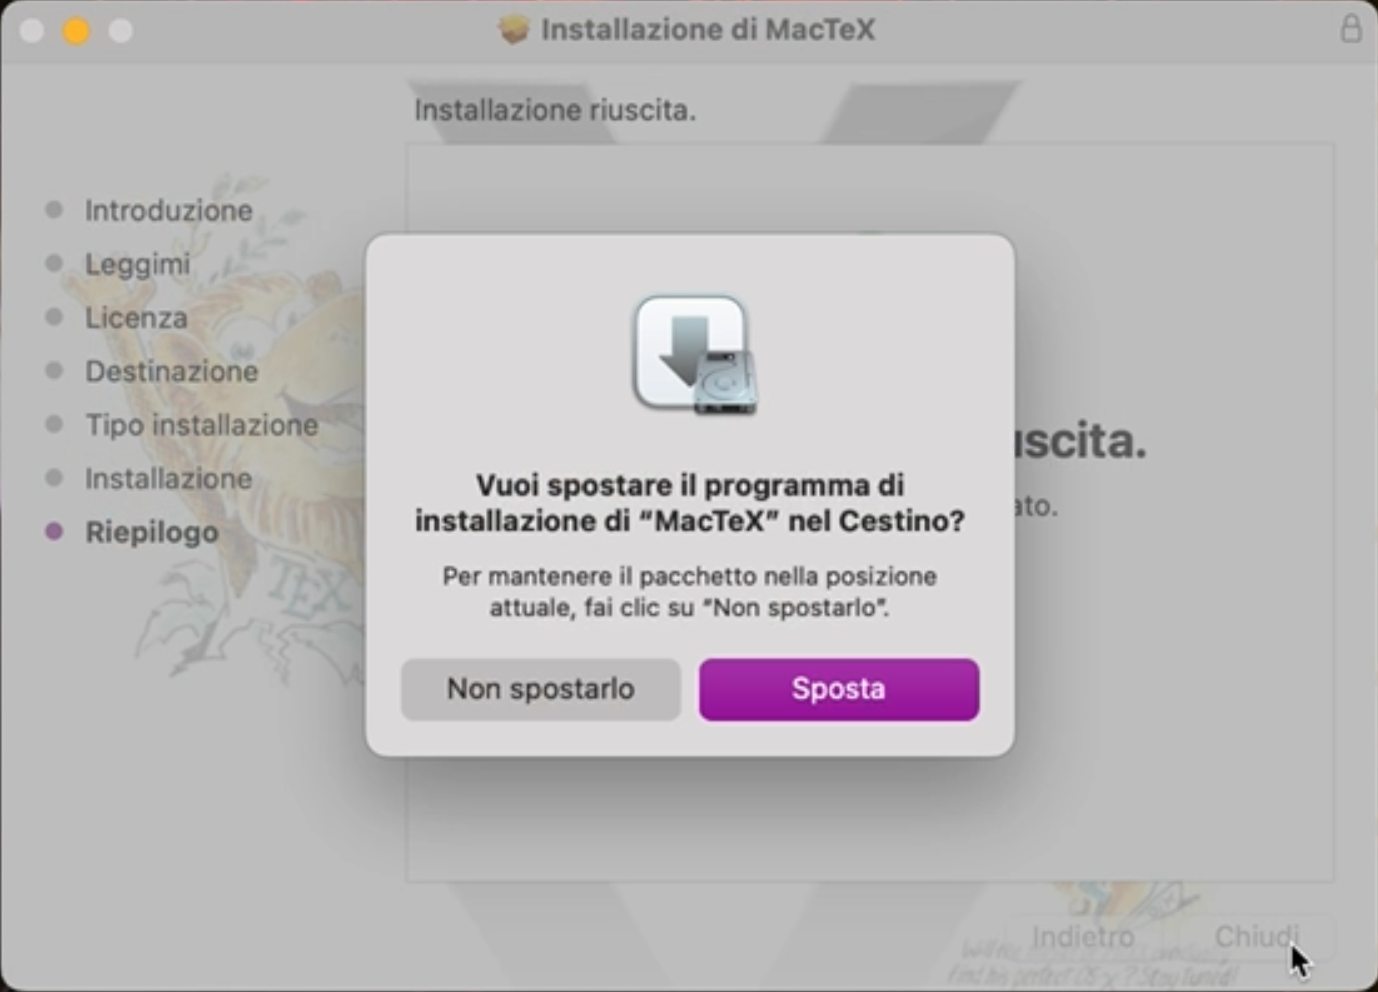
\includegraphics[width=0.9\linewidth]{images/texlive/mac/8_eliminazione_installer.png}
    \caption{MacTeX: Eliminazione installer}
    \label{mactex_eliminazione_installer}
\end{figure}

\subsubsection{Risoluzione dei problemi}
\begin{itemize}

    \item \label{enoent} Nel caso in cui la compilazione dei documenti dovesse dare un errore di tipo ENOENT, è necessario aggiungere il compilatore al PATH,
        per farlo aprire un terminale e scrivere:
        %gobble rimuove i primi n caratteri dalle righe, permettendo 
        % così di indentare il codice in LaTeX
        %autogobble rimuove automaticamente gli spazi, preservando l'indentazione
        \begin{minted}[gobble=10]{zsh}
            nano $HOME/.zshrc
        \end{minted}
        Nel file che si apre aggiungere alla fine la riga
        \begin{minted}[gobble=10]{zsh}
            export PATH="/usr/local/texlive/2024/bin/universal-darwin:$PATH"
        \end{minted}
        Per sicurezza verificare il percorso, perchè la cartella {\tt 2024} cambia in base alla versione, mentre la cartella {\tt universal-darwin} cambia in base, non solo alla versione, ma anche all'architettura del processore.

        Dopo questo passaggio è consigliabile chiudere COMPLETAMENTE Visual Studio Code dal menù in alto a sinistra e riaprirlo, se non dovesse risolvere, riavviare il computer.


    \item A volte, l'installatore visualizza una finestra di dialogo che dice “Verifica...” e poi l'installazione si blocca. In tutti i casi conosciuti, il riavvio del Macintosh risolve il problema. Dopo il riavvio, eseguire nuovamente l'installazione.

    \item Se durante l'installazione vengono segnalati altri problemi, riferirsi alla sezione \href{https://www.tug.org/mactex/mactex-download.html}{“Errori di installazione”} della guida ufficiale.

    \item MacTeX scrive un collegamento simbolico /Library/TeX/texbin che punta alla directory dei binari di TeX Live. Configurare i programmi GUI per utilizzare questo collegamento. I programmi GUI forniti si configurano automaticamente.
    
\end{itemize}

Questa che hai appena letto è una sotto-sottosezione.

Non ti sono bastati 3 livelli?

\href{https://tex.stackexchange.com/questions/60209/how-to-add-an-extra-level-of-sections-with-headings-below-subsubsection}{Questo è un link per stackexchange, spiega come aggiungere altri livelli di sottosezioni.}

\subsection{Linux e Unix}
Per voi uomini coraggiosi che non avete paura di usare un terminale, propongo i comandi per l'installazione su distribuzioni Debian-based:
\begin{minted}{bash}
    sudo apt install texlive-science texlive-latex-extra latexmk \
        texlive-extra-utils texlive-publishers texlive-science
\end{minted}

\section{Visual Studio Code}
Per la scrittura si userà Visual Studio Code, editor multipiattaforma estensibile con numerosi plug-in.
D'ora in poi ci si riferirà ad esso col suo nome breve: vscode.

\subsection{Installazione}
\subsubsection{Windows, MacOS e distribuzioni Linux senza snap}
Per l'installazione su queste piattaforme si consiglia di seguire direttamente il sito del programma \url{https://code.visualstudio.com/download}.

\subsubsection{Distribuzioni con snap}
\begin{minted}{bash}
    sudo snap install code --classic
\end{minted}

\subsection{Configurazione}
Installato Visual Studio Code e completata la configurazione iniziale (opzionale),
la schermata presentata sarà simile a questa.
\begin{figure}[H]
    \centering
    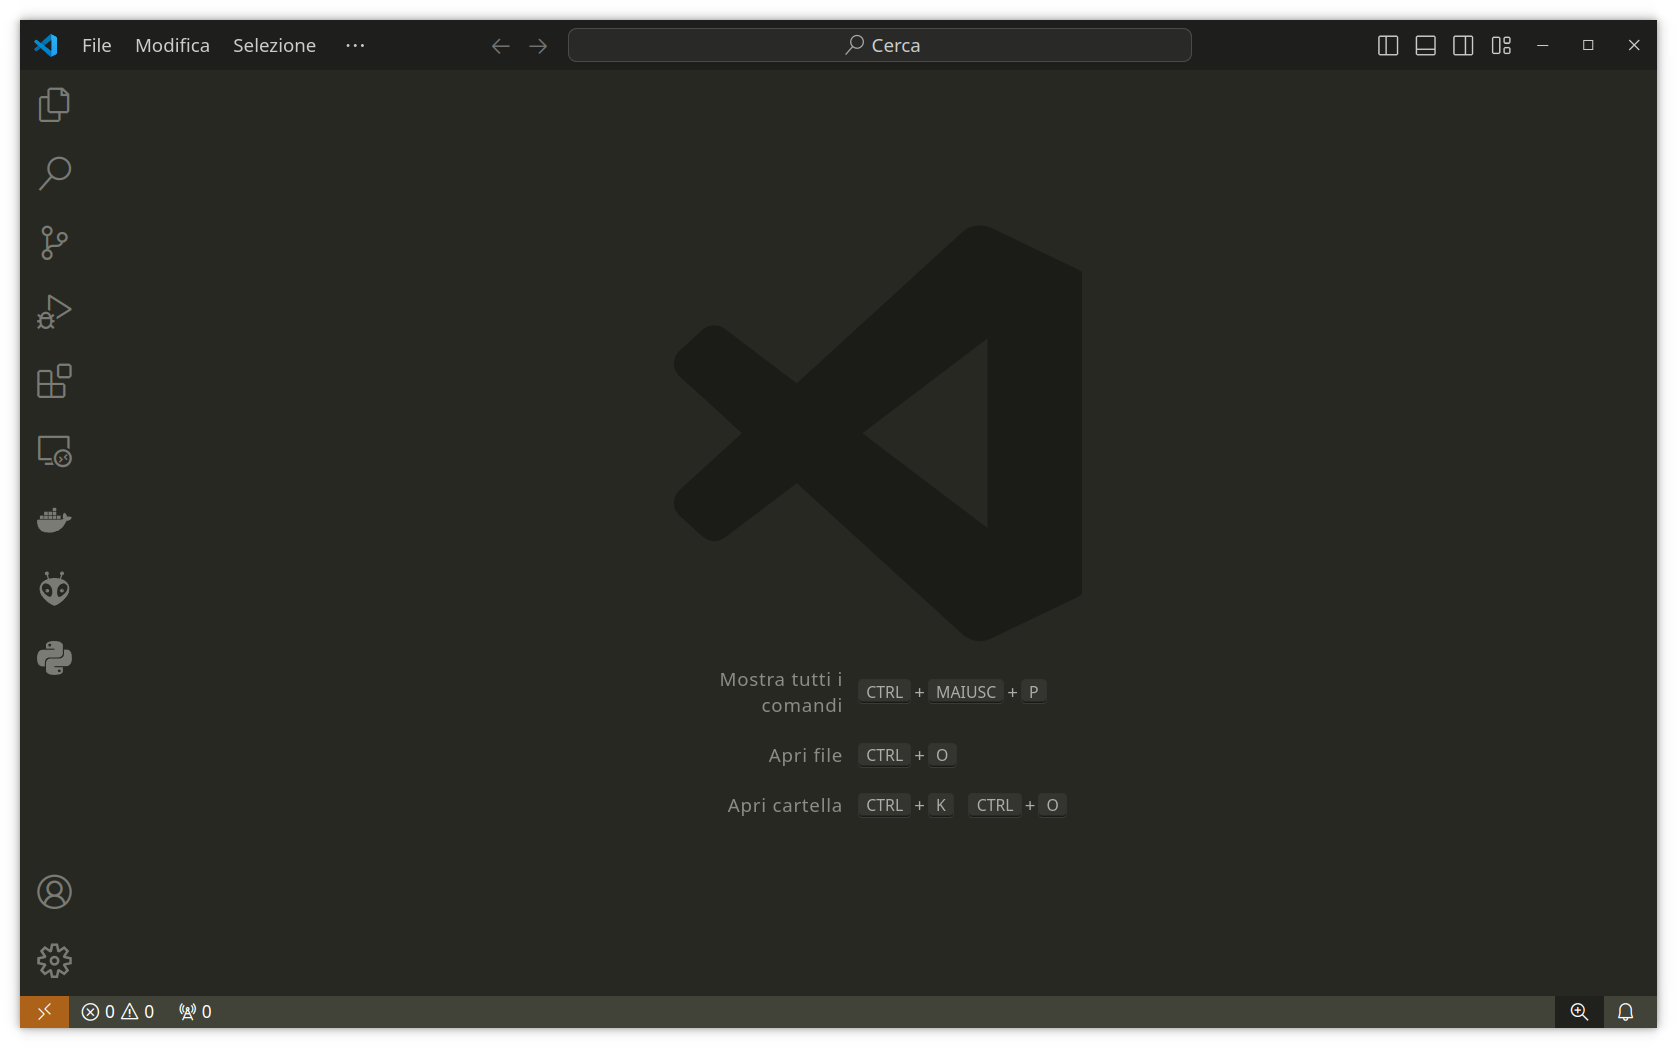
\includegraphics[width=\linewidth]{images/vscode/vscode.png}
    \caption{Schermata iniziale di vscode}
    \label{schermata_iniziale_vscode}
\end{figure}
Cliccare su 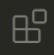
\includegraphics[height=5mm]{images/vscode/estensioni_icona.png}
per aprire il menu delle estensioni.
\begin{figure}[H]
    \centering
    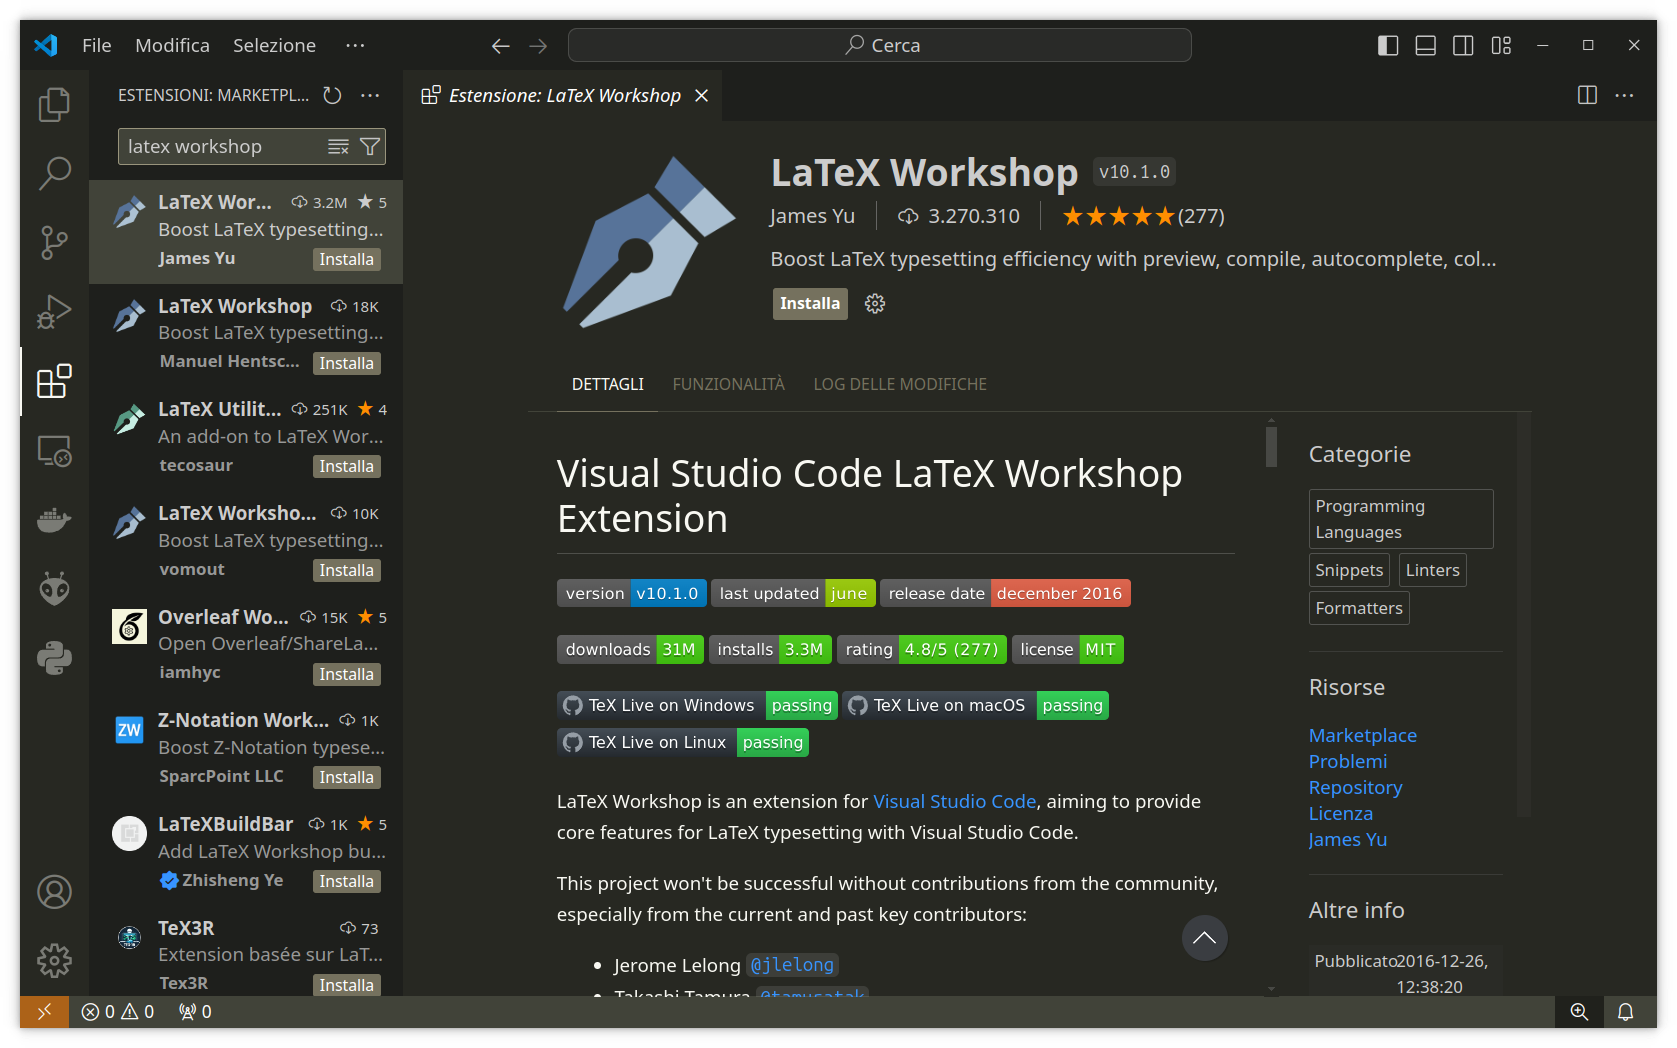
\includegraphics[width=\linewidth]{images/vscode/vscode_latex_workshop.png}
    \caption{Schermata gestore estensioni}
    \label{schermata_gestore_estensioni}
\end{figure}
Nella barra di ricerca cercare Latex Workshop e premere su installa per avviare l'installazione.
Terminata l'installazione aprire il menu delle azioni rapide con Ctrl + Alt + P (Cmd + Alt + P su MacOS).
\begin{figure}[H]
    \centering
    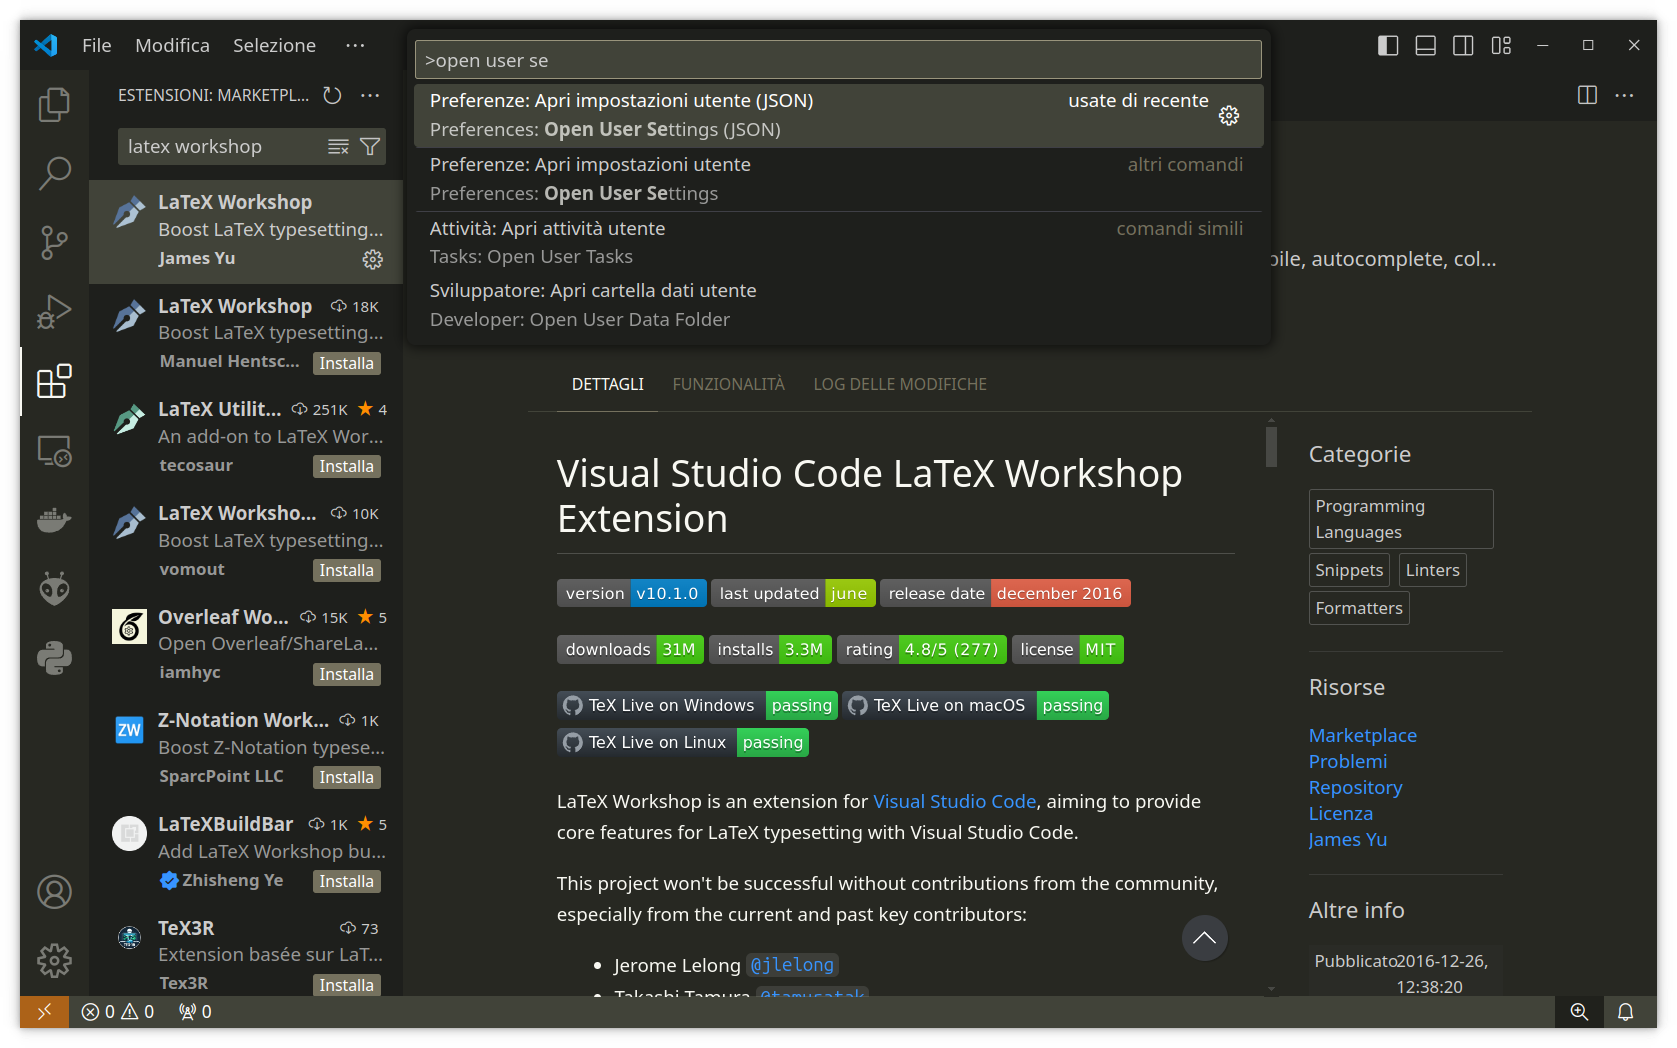
\includegraphics[width=\linewidth]{images/vscode/vscode_user_settings.png}
    \caption{Menu azioni rapide}
    \label{menu_azioni_rapide}
\end{figure}
Cercare "Open User Settings (JSON)" come in figura \ref{menu_azioni_rapide} e selezionare la voce.
\begin{figure}[H]
    \centering
    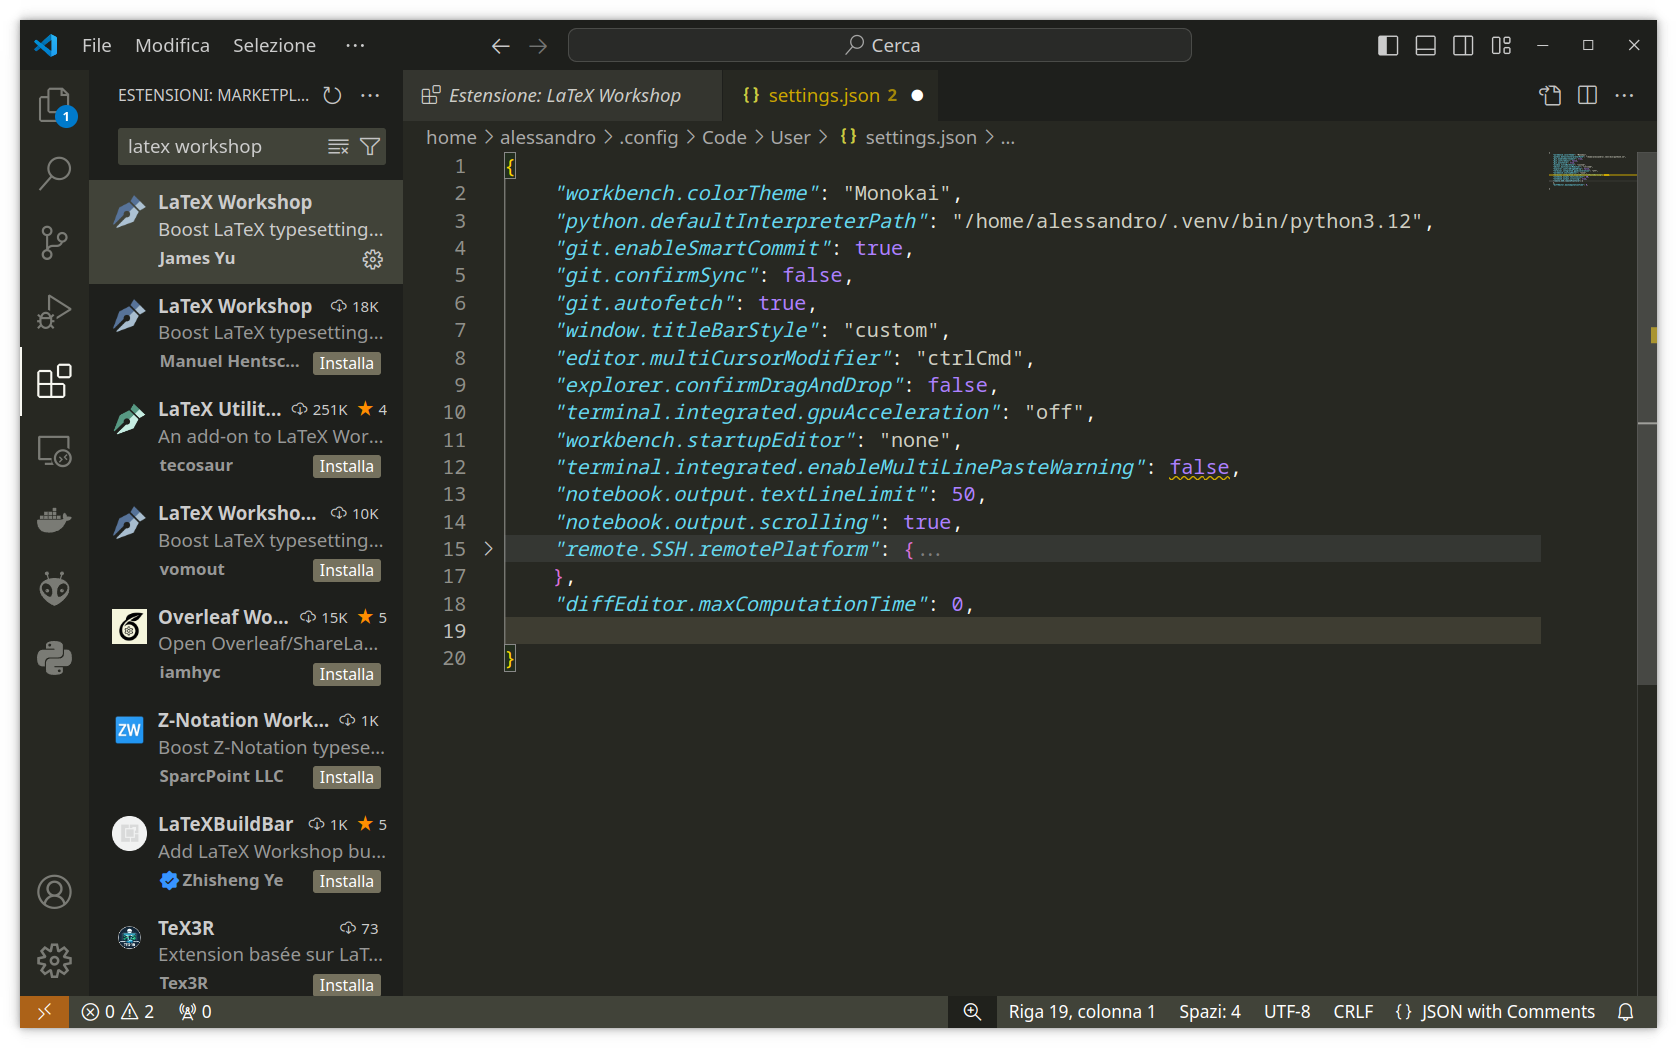
\includegraphics[width=\linewidth]{images/vscode/vscode_settings_json.png}
    \caption{File JSON delle impostazioni}
    \label{json_impostazioni}
\end{figure}
Nella schermata che si apre incollare il contenuto del file my\_settings.json presente nella cartella del progetto.
È possibile eliminare il file dopo aver inserito il suo contenuto nel file settings.json di vscode.\\
ATTENZIONE: Il file che si sta modificando è un file JSON, in quanto tale richiede alcuni semplici accorgimenti di sintassi.
Se, come nella figura \ref{json_impostazioni}, sono già presenti altre righe, dopo l'ultima è necessario aggiungere una virgola prima di incollare il resto delle impostazioni.

Il risultato finale dovrebbe essere qualcosa di simile a \ref{json_impostazioni_nuovo}
\begin{figure}[H]
    \centering
    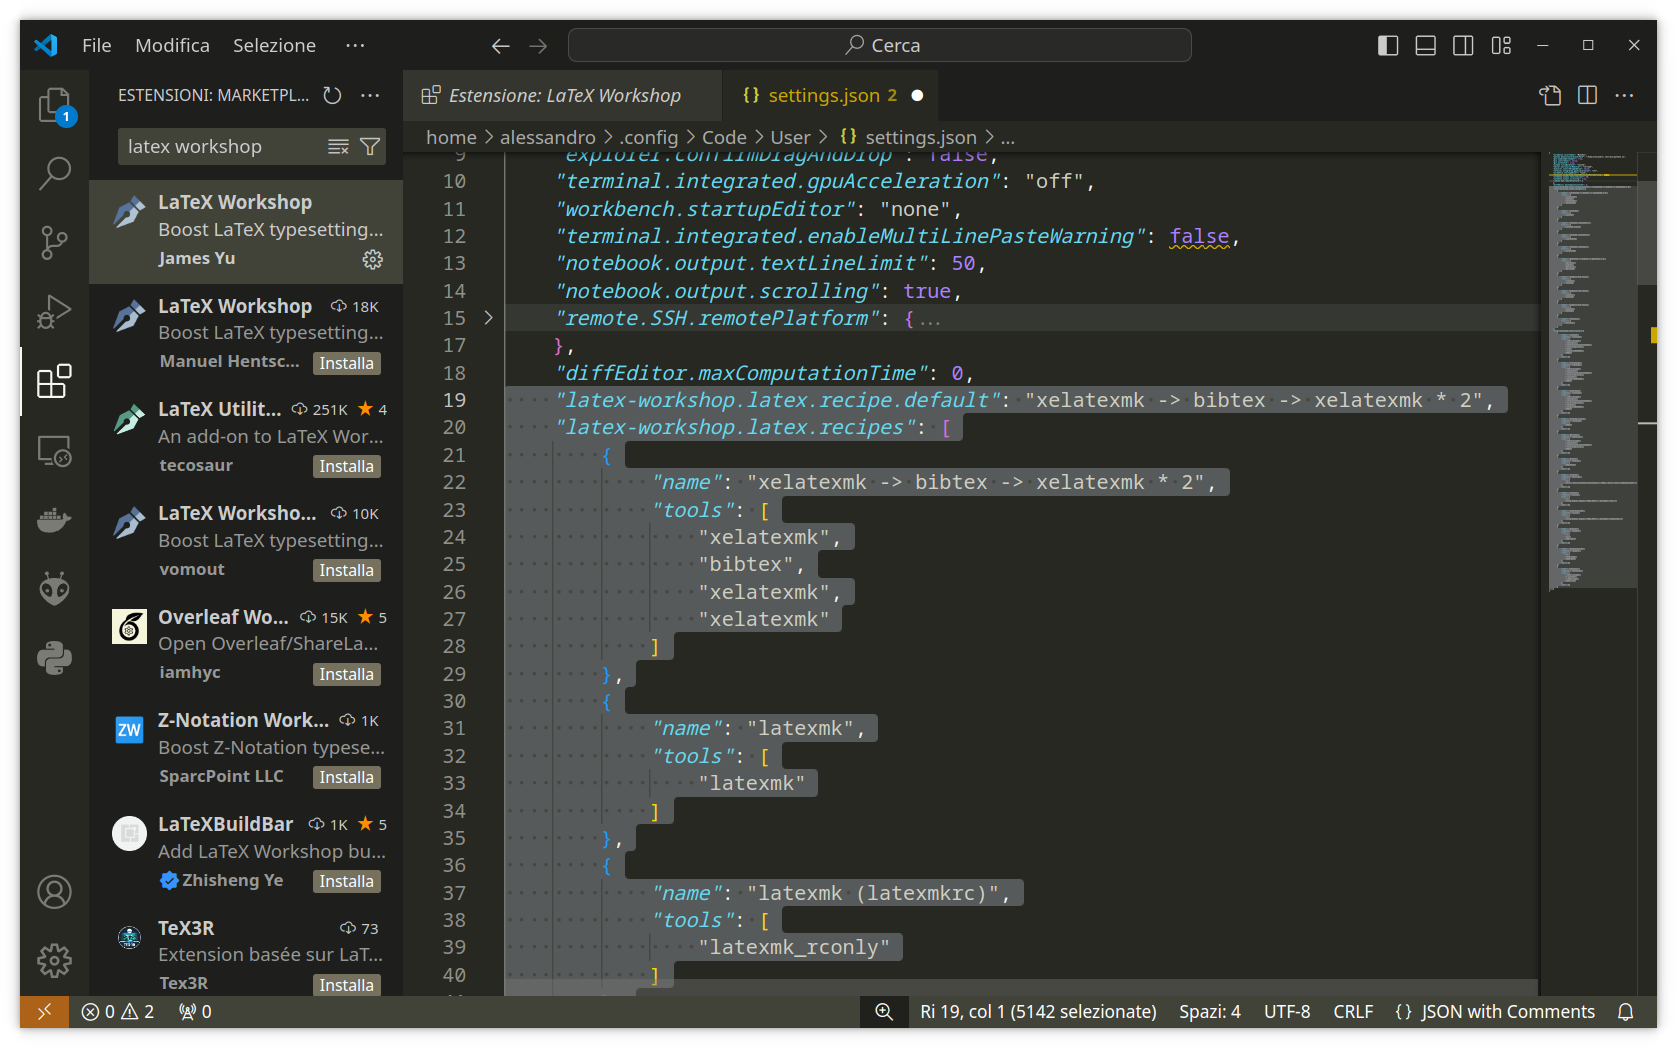
\includegraphics[width=\linewidth]{images/vscode/vscode_settings_json2.png}
    \caption{File JSON delle impostazioni dopo la modifica}
    \label{json_impostazioni_nuovo}
\end{figure}




% \section{È il momento delle figure}

% \LaTeX adora spostare le figure, quindi bisognerà un po' giocare col testo per trovare la posizione adatta.


% \begin{figure}[h]
%     \centering 
%     
\includegraphics[width=0.2\linewidth]{logodiceam.png} 
%     \caption{Per comodità useremo il logo del dipartimento DICEAM.}
%     \label{figura_logo_diceam}
% \end{figure}

% In generale è consigliabile lasciar fare tutto al compilatore e poi referenziare la figura così \ref{figura_logo_diceam}. \citep{forceFigurePlacement}

% Se proprio è necessario posizionare l'immagine in una posizione precisa, usare [H] invece di [h].

% \section{Syntax highlighting}
% Se a qualcuno piacesse scrivere codice e magari renderlo leggibile, minted fa al caso suo.
% Altri stili: \\
% \url{https://www.overleaf.com/learn/latex/Code_Highlighting_with_minted}

% \begin{minted}{python}
% import numpy as np
    
% def incmatrix(genl1,genl2):
%     m = len(genl1)
%     n = len(genl2)
%     M = None #to become the incidence matrix
%     VT = np.zeros((n*m,1), int)  #dummy variable
    
%     #compute the bitwise xor matrix
%     M1 = bitxormatrix(genl1)
%     M2 = np.triu(bitxormatrix(genl2),1) 

%     for i in range(m-1):
%         for j in range(i+1, m):
%             [r,c] = np.where(M2 == M1[i,j])
%             for k in range(len(r)):
%                 VT[(i)*n + r[k]] = 1;
%                 VT[(i)*n + c[k]] = 1;
%                 VT[(j)*n + r[k]] = 1;
%                 VT[(j)*n + c[k]] = 1;
                
%                 if M is None:
%                     M = np.copy(VT)
%                 else:
%                     M = np.concatenate((M, VT), 1)
                
%                 VT = np.zeros((n*m,1), int)
    
%     return M
% \end{minted}

\chapter{Controllo versione} \label{Cap.2}

\vspace{2cm}

\begin{flushright}
\textit{Breve introduzione al sistema di controllo versione\\ per sincronizzazione dei file del documento su GitHub.}
\end{flushright}

\vspace{0.5cm}

La scrittura di un lavoro di tesi richiede tempo ed è consigliabile che questo documento non esista in una sola copia,
per evitare disastri e per poter lavorare da più dispositivi (se necessario), è altamente consigliabile usare un software
di controllo verione per poter sempre avere traccia delle modifiche e sincronizzarle con un server remoto all'occorrenza.

Per svolgere questo compito ci si avvarrà del programma git e del servizio GitHub.

\section{Git}
Git è un client che permette la creazione e gestione di repository.
\subsection{Installazione \citep{installGit}}
In base alle prove effettuate, risulta già installato su MacOS, quindi questo non verrà documentato.
\subsubsection{Windows}
Cliccando col tasto destro sull'icona di Start, a seconda della versione del sistema operativo e della configurazione, cliccare su:
\begin{itemize}
    \item Apri Powershell (Amministratore)
    \item Apri Prompt dei comandi (Amministratore)
    \item Apri Terminale (Amministratore)
\end{itemize}
Nel prompt scrivere {\tt winget install git.git}, accettare con {\tt y} e invio quando chiede conferma.

\subsubsection{Linux}
Anche in questo caso l'installazione dipende da distribuzione a distribuzione. Per le distribuzioni Debian-based, il comando è il seguente:
\begin{minted}{bash}
    sudo apt install git
\end{minted}

\subsection{Configurazione}
Per poter usare Git è necessario specificare nome e email dell'utente che lo userà.
Sempre nel terminale inserire questi due comandi (validi per tutte le piattaforme) opportunamente modificati con i vostri dati, è molto 
importante prestare attenzione alle virgolette attorno a nome e email:
\begin{minted}{bash}
    git config --global user.name "Mario Rossi"
    git config --global user.email "mario.rossi@unirc.it"
\end{minted}

\section{GitHub}
\begin{wrapfigure}{l}{0.10\textwidth}
    \centering
    \vspace{-0.5\linewidth} % Rimuove lo spazio bianco prima della figura
    
\includegraphics[width=\linewidth]{images/github/github.png}
    \vspace{-0.9\linewidth} % Rimuove lo spazio bianco dopo della figura
    %\caption{Logo GitHub}
    \label{logo_github}
\end{wrapfigure}

GitHub è un servizio di hosting per progetti software, che implementa lo strumento di controllo versione distribuito Git.
Recandosi alla pagina \url{https://github.com} è possibile registrarsi o accedere al proprio account, per poter creare
un proprio fork\footnote{Nell'ambito dell'ingegneria del software e dell'informatica, indica lo sviluppo di un nuovo progetto 
software che parte dal codice sorgente di un altro già esistente, a opera di un programmatore.} di questo progetto.

La registrazione è una procedura triviale e non è necessario documentarla.

Recarsi alla pagina \url{https://github.com/a13ssandr0/TesiUnirc} e premere il pulsante {\tt Fork} in alto a destra.
\begin{figure}[H]
    \centering
    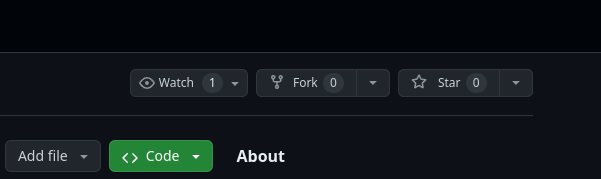
\includegraphics[width=\linewidth]{images/github/fork.png}
    \caption{Pulsante fork}
    \label{pulsante_fork}
\end{figure}

Nella pagina che appare dare un nome alla repository\footnote{Una repository è la cartella principale in cui vengono salvati i file.}
e concludere con Create fork.
\begin{figure}[H]
    \centering
    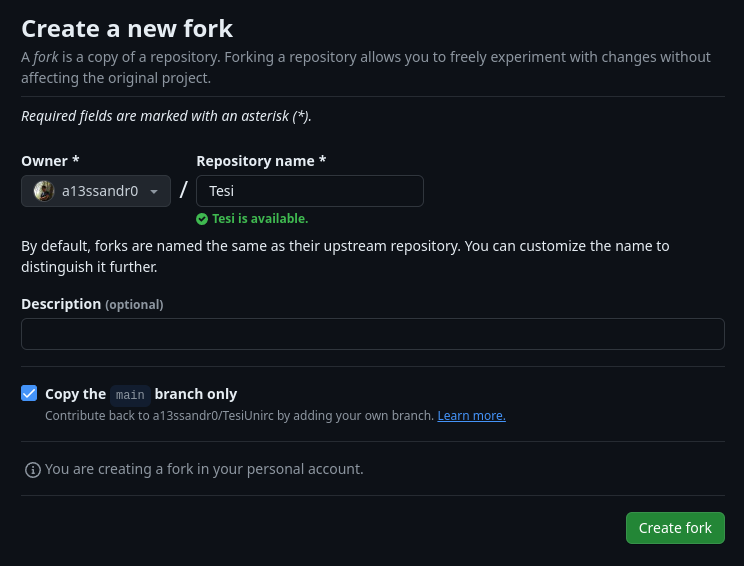
\includegraphics[width=\linewidth]{images/github/new_fork.png}
    \caption{Pagina creazione fork}
    \label{pagina_fork}
\end{figure}

\newpage

\section{Visual Studio Code}
Creata la repository personale, è possibile clonarla in vscode. \citep{vscodeGit}
\begin{figure}[H]
    \centering
    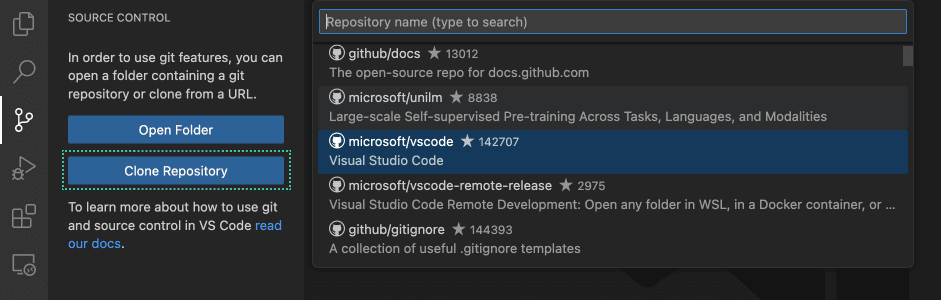
\includegraphics[width=\linewidth]{images/vscode/vscode_clone_repo.png}
    \caption{Menu clonazione repository}
    \label{clonazione_repository}
\end{figure}
La prima volta, prima di far selezionare la repository chiederà di accedere con il proprio account GitHub.
Inserire il nome della propria repository per clonarla, premere invio e selezionare la cartella in cui clonarla.
Vscode automaticamente la scaricherà e aprirà il progetto.

Se tutto è stato configurato correttamente, aprendo il file book.tex comparirà un triangolo verde in alto 
a destra per compilare il documento e creare il pdf, in generale il progetto viene
ricompilato automaticamente ad ogni salvataggio del file.

Su MacOS è molto probabile che all'esecuzione del compilatore venga restituito un errore ENOENT,
fare riferimento al primo punto della sezione Risoluzione dei problemi a pagina \pageref{enoent}.



\chapter{Esempi}  \label{Cap.3}

\vspace{2cm}

\begin{flushright}
 \textit{Altri esempi di scrittura in \LaTeX\ che non è stato possibile inserire nei capitoli precedenti.}
\end{flushright}

\vspace{0.5cm}



Testo multicolonna: 

\begin{multicols}{2}
    \textbf{Colonna 1}\\
    Testo della prima colonna.
\columnbreak\\
    \textbf{Colonna 2}\\
    Non lo scrivo nemmeno.
\end{multicols}


Signore e signori, sua maestà l'elenco numerato:
\begin{enumerate}
    \item Lorem
    \item Ipsum
    \item Dolor
    \item Sit
    \item Amet
    \item Sì ho avuto molta fantasia
\end{enumerate} 

%questo abominio serve per forzare latex a saltare una riga
\ \\

Per forzare uno o più spazi bisogna usare uno o più backslash, ognuno seguito da uno spazio.\\
Testo normale\\
Testo \ con uno spazio\\
Testo \ \ con due spazi\\
Testo \ \ \ con tre spazi

Un elenco di elenchi??

Roba degna del più forte elencatore d'Italia. \citep{elencatoreSeriale}
\begin{itemize}
    \item \textbf{A}: AAAA
    \begin{itemize}
        \item Aa
        \item Ab
        \item Ac
        \item Ad
        \item Ae
        \item Af
    \end{itemize} 
    \item \textbf{B}: BBBB
    \begin{itemize}
        \item Ba
        \item Bb
        \item Bc
        \item Bd
        \item Be
        \item Bf
    \end{itemize}
\end{itemize}

\newpage
newpage termina la pagina attuale e inizia una nuova pagina.

\vspace*{2cm}

Non avevamo ancora parlato delle tabelle.

Sono lunghe da trattare quindi lasciamo il duro compito alla documentazione di Overleaf.
\url{https://www.overleaf.com/learn/latex/Tables}

\begin{table}[h!]
\centering
\begin{tabular}{||c c c c||} 
    \hline
    Col1 & Col2 & Col2 & Col3 \\ [0.5ex] 
    \hline\hline
    1 & 6 & 87837 & 787 \\ 
    2 & 7 & 78 & 5415 \\
    3 & 545 & 778 & 7507 \\
    4 & 545 & 18744 & 7560 \\
    5 & 88 & 788 & 6344 \\ [1ex] 
    \hline
\end{tabular}
\caption{Table to test captions and labels.}
\label{table:1}
\end{table}


\newpage
\begin{landscape}
landscape mette il contenuto della pagina in orizzontale.
\end{landscape}
    


\chapter*{Conclusioni}
\addcontentsline{toc}{chapter}{Conclusioni}
\markboth{Conclusioni}{Conclusioni}

\vspace{2cm}

\begin{flushright}
 \textit{<SINTESI DELLE CONCLUSIONI>}
\end{flushright}

\vspace{0.5cm}

Le conclusioni funzionano come tutti gli altri capitroli.

Come l'introduzione questo capitolo non ha il numero.

\section*{Sezione delle conclusioni}
La sezione con l'asterisco non ha il numero.

\chapter*{Ringraziamenti}
\addcontentsline{toc}{chapter}{Ringraziamenti}
\markboth{Ringraziamenti}{Ringraziamenti}

Ringrazio il dipartimento DIIES per aver pubblicato un modello di tesi non troppo aggiornato.

Ringrazio Alessandro Campolo\footnote{``ringrazio me stesso" è poco radiofonico.} \footnote{e così abbiamo scoperto anche le note a piè di pagina.}
per aver aggiornato il modello e scritto la documentazione per installare tutti i programmi per lavorare al documento.

Ringrazio Gemma Pia Romeo per aver fornito la sua tesi come punto di partenza per gli esempi presenti in queste pagine.




\bibliographystyle{apalike}
\bibliography{biblio}

\end{document} 